\cleardoublepage
\chapter{Trialling of alternative cDNA synthesis approaches}\label{ch:alt_cDNA}

\stoptocwriting
\section{Alternative cDNA synthesis approaches}
Despite the power of the SMARTer cDNA synthesis kit (Clontech) to enrich for high-quality and full-length cDNA templates, this kit is costly and fails to differentiate between intact and degraded RNA (as described in \cref{section:ch2_cDNA_synthesis_explanation}). Two alternative methods were therefore trialled and optimised on a mouse cortical sample:
\begin{enumerate}
	\item An adaptation of the cDNA synthesis protocol (provided by J. Ragoussis) taken from the “Wellcome Trust Advanced Course: RNA Transcriptomics (2018)” (hereby referred to as “WTAC”) which I attended during my PhD. This protocol is based on the Smart-seq2 protocol\cite{Picelli2014}, which formed the basis for the SMARTer cDNA synthesis kit. 
	\item Full-Length cDNA Amplification (TeloPrime) kit, which ensured the amplification of fully-intact cDNA containing the 5' cap.    
\end{enumerate}

Unfortunately, I was unable to generate sufficient cDNA material from the Full-Length cDNA Amplification kit required for downstream library preparation. The following section thus only documents the optimised protocol and results from the adaptation of the WTAC protocol, based on Smart-seq2.

\subsection{Adaptation of Smart-seq2}
In the WTAC protocol, SuperScript IV enzyme (SSIV) was used for reverse transcription of RNA into cDNA due to its high thermal-stability, subsequently allowing it to be used in high temperatures to resolve complex RNA secondary structures. Reverse transcription step was also split into two steps, pre-RT and RT, to first hybridise poly(T) primer to poly(A) tract of mRNA before first-strand synthesis (\cref{WTAC_Pre_RT_Mix} - \cref{WTAC_RT_incubation}). cDNA templates were then amplified using Advantage 2 high fidelity polymerase.

One of the challenges in applying the WTAC protocol to the mouse experiments was the high amount of RNA needed for cDNA synthesis: 300ng/$\mu$L was specified as the starting amount, but majority of the samples only had an average concentration of 70ng/$\mu$L. The volume of pre-RT and RT PCR mix was therefore upscaled to account for additional sample volume, while maintaining the concentration of other reagents. 

\subsubsection{Protocol}

\vspace{1cm}
\begin{table}[h]
	\setlength\tabcolsep{6pt} %reduced margin size in table
	\caption[List of reagents for Smart-seq2]%
	{\textbf{List of reagents for Smart-seq2 protocol}}
	\label{reagents}
	\begin{tabularx}{0.95\textwidth}{lcc}
		\toprule
		Reagents                                                      & Supplier (Catalogue)                                  & Step                 \\ \midrule
		ERCC RNA Spike-In Mix                                         & Thermo Fisher Scientific (4456740)                    & Pre-RT               \\
		RNAse inhibitor (40 U/$\mu$L)                                     & Clontech (2313A)                                      & Pre-RT               \\
		\begin{tabular}[c]{@{}l@{}}Advantage UltraPure PCR dNTP Mix \\ (10 mM each dNTP)\end{tabular} & Clontech (639125)                                     & Pre-RT               \\
		\tabitem SuperScript IV (200U/$\mu$L)                                      & \multirow{3}{*}{Thermo Fischer Scientific (18090010)} & RT                   \\
		\tabitem 5X RT Buffer                                                  &                                                       & Pre-RT               \\
		\tabitem DTT (0.1M)                                                    &                                                       & RT                   \\
		Betaine (5M)                                                  & Sigma-Aldrich (B0300-1VL)                             & RT                   \\
		MgCl2 (1M)                                                    & Thermo Fisher Scientific (AM9530G)                    & RT                   \\
		10X Advantage 2 PCR Buffer                                    & \multirow{3}{*}{Clontech (639207)}                    & \multirow{3}{*}{PCR} \\
		50X Advantage 2 Polymerase Mix                                &                                                       &                      \\
		50X dNTP Mix                                                  &                                                       &                      \\ \cmidrule(r){1-3}
	\end{tabularx}
\end{table}

\begin{enumerate}
	\item Assuming a stock ERCC RNA spike-in concentration of 30.3ng/$\mu$L and a final concentration of 1.8ng/$\mu$L, 1$\mu$L of stock ERCC RNA spike-in was originally diluted with 15.83 TE buffer (dilution of 1:16.83). 
	\item Pre-reverse transcription PCR mix was prepared with RNA (\cref{WTAC_Pre_RT_Mix}).
	\item The sample was mixed by tapping the tube, spun down and incubated in the conditions outlined in \cref{WTAC_Pre_RT_incubation} to prime the RNA with poly(T).
	\item Reverse transcription PCR mix was prepared with primed-RNA (\cref{WTAC_RT_Mix}).
	\item The sample was mixed by tapping the tube, spun down and incubated in the conditions outlined in \cref{WTAC_RT_incubation} for first-strand cDNA synthesis.
	\item cDNA from RT reaction was split into 7 PCR tubes, each with 1$\mu$L of cDNA and reagents tabulated in \cref{WTAC_PCR_Mix}.
		\begin{itemize}
			\item This step was necessary to test the optimal number of PCR cycles to prevent over-amplification, with the PCR tubes incubated for different cycle durations.
		\end{itemize}
	\item All 7 PCR tubes were incubated simultaneously (\cref{WTAC_PCR_Incubation}), with one PCR tube removed at each cycle from cycle 12 to cycle 18 in segment 3 (as suggested by WTAC protocol) and placed in ice.
	\item At the end of segment 3 in \cref{WTAC_PCR_Incubation}, all 6 PCR tubes were placed back into the thermal cycler for enzyme termination (\cref{WTAC_PCR_Incubation}, segment 4). 
	\item PCR tubes were analysed on a 1\% agarose gel (described in \cref{Isoseq_Protocol_running_agarose_gel}) or on a D5000 genomic ScreenTape (described in \cref{Isoseq_Protocol_tapestation_bioanalyzer}).	
\end{enumerate}

\vspace{1cm}
\begin{table}[h]
	\centering
	\captionsetup{width=0.95\textwidth}
	\caption[Pre-reverse transcription PCR mix]%
	{\textbf{Pre-reverse transcription PCR mix.} Tabulated is a list of the reagent volume from the WTAC protocol, and of that optimised to use a lower initial RNA concentration. While the \textit{total volume per Sample} was different due to amount of RNA used (200ng), the final concentrations of all the other remaining reagents were maintained.}
	\label{WTAC_Pre_RT_Mix}
	\setlength\tabcolsep{8pt} %reduced margin size in table
	\begin{tabularx}{0.95\textwidth}{lccc}
		\toprule
		\multirow{2}{*}{Reagents} & \multirow{2}{*}{\begin{tabular}[c]{@{}c@{}}Final\\ concentration\end{tabular}} & \multicolumn{2}{c}{Volume ($\mu$L/sample)}      \\ \cmidrule(l){3-4} 
		&                                                                                & WTAC protocol & Optimised protocol \\ \cmidrule(r){1-4}
		Diluted ERCC RNA            &                                                                                & 0.1                    & 0.1                \\
		Rnase Inhibitor             & 0.64U/$\mu$L                                                                       & 0.05                   & 0.08               \\
		Poly(T) primer               & 2.76$\mu$M                                                                         & 0.7                    & 1.15               \\
		SuperScript IV Buffer       & 0.17                                                                           & 0.1                    & 0.17               \\
		Nuclease-Free Water                        &                                                                                & 0                      & 0.55               \\
		dNTP Mix                    & 1.9mM                                                                          & 0.56                   & 0.95               \\
		Total RNA                   &                                                                                & 1.5 (300ng)                    & 2 (200ng)                 \\
		\textit{Total volume per Sample}            &                                                                                & \textit{3}                      & \textit{5}                  \\ \bottomrule
	\end{tabularx}
\end{table}

\vspace{1cm}
\begin{table}[h]
	\centering
	\captionsetup{width=0.95\textwidth}
	\caption[PCR conditions for pre-reverse transcription]%
	{\textbf{PCR conditions for pre-reverse transcription.} Tabulated are the PCR conditions for amplification of cDNA templates: initial 72°C to prompt unfolding of RNA secondary structures, 4°C for poly(T) binding and 25°C to encourage more specific binding.}
	\setlength\tabcolsep{6pt} %reduced margin size in table
	\label{WTAC_Pre_RT_incubation}
	\begin{tabularx}{0.95\textwidth}{
			>{\centering\arraybackslash}X 
			>{\centering\arraybackslash}X 
			>{\centering\arraybackslash}X}
		\toprule
		Segments & Temperature (°C) & Time (minutes) \\ \midrule
		1        & 72               & 3             \\
		2        & 4                & 10             \\
		3        & 25               & 1                   \\ \bottomrule
	\end{tabularx}
\end{table}


\begin{table}[h]
	\centering
	\captionsetup{width=0.95\textwidth}
	\setlength\tabcolsep{7pt} %reduced margin size in table
	\caption[Reverse transcription PCR mix]%
	{\textbf{Reagent composition for reverse transcription PCR mix.}}
	\label{WTAC_RT_Mix}
	\begin{tabularx}{0.95\textwidth}{lccc}
		\toprule
		\multirow{2}{*}{Reagents}            & \multirow{2}{*}{\begin{tabular}[c]{@{}c@{}}Final\\ concentration\end{tabular}} & \multicolumn{2}{c}{Volume ($\mu$L/sample)}      \\ \cmidrule(l){3-4} 
		&                                                                                &  WTAC protocol & Optimised protocol \\ \cmidrule(r){1-4}
		Sample from pre-RT                   &                                                                                & 3                      & 5                  \\
		dH20                                 &                                                                                & 0.85                   & 0.55               \\
		Superscript IV Buffer                & 1.00 U/$\mu$L                                                                      & 0.8                    & 1.1                \\
		DTT                                  & 0.57 mM                                                                         & 0.175                  & 0.25               \\
		TSO                                  & 2.50 mM                                                                        & 0.7                    & 1                  \\
		RNAse inhibitor                      & 1.20 uM                                                                        & 0.175                  & 0.25               \\
		SuperScript IV RT & 10.0 U/$\mu$L                                                                      & 0.35                   & 0.5                \\
		Betaine                              & 0.50 M                                                                         & 0.7                    & 1                  \\
		MgCl2                                & 3.57 mM                                                                        & 0.25                   & 0.35               \\
		\textit{Total volume per sample}              &                                                                                & \textit{7}                      & \textit{10}                 \\ \bottomrule
	\end{tabularx}
\end{table}


\begin{table}[h]
	\centering
	\captionsetup{width=0.95\textwidth}
	\caption[PCR conditions for reverse transcription]%
	{\textbf{PCR conditions for reverse transcription.} Tabulated is a list of the PCR conditions as taken from the WTAC protocol. Segments 2, 3, 5, 7, 9 allow the unfolding of RNA secondary structures and completion or continuation of RT with successive higher temperatures, whereas segments 1, 4, 6 and 8 allow template switching. Segment 11 is for enzyme termination.}
	\label{WTAC_RT_incubation}
	\begin{tabularx}{0.95\textwidth}{
			>{\centering\arraybackslash}X
			>{\centering\arraybackslash}X 
			>{\centering\arraybackslash}X  
			>{\centering\arraybackslash}X}
		\toprule
		Segments & Temperature (°C) & Time   & Cycles \\ \midrule
		1        & 50          & 10 minutes & 1      \\
		2        & 55          & 30 seconds & 10     \\
		& 50          & 30 seconds &        \\
		3        & 60          & 30 seconds & 5      \\
		& 55          & 30 seconds &        \\
		4        & 50          & 30 seconds & 1      \\
		5        & 60           & 30 seconds & 5      \\
		& 60          & 30 seconds &        \\
		6        & 50          & 30 seconds & 1      \\
		7        & 70          & 30 seconds & 5      \\
		& 65          & 30 seconds &        \\
		8        & 50          & 30 seconds & 1      \\
		9        & 75          & 30 seconds & 5      \\
		& 70          & 30 seconds &        \\
		10       & 50          & 1 minute  & 1      \\
		11       & 80          & 10 minutes & 1      \\ \bottomrule
	\end{tabularx}
\end{table}


\begin{table}[h]
	\centering
	\captionsetup{width=0.95\textwidth}
	\caption[PCR Mix]%
	{\textbf{PCR Mix.} Tabulated is a list of the reagent volumes as taken from the WTAC protocol. The volume tabulated is sufficient for only 1$\mu$L of cDNA from total RT reaction - upscale accordingly.}
	\label{WTAC_PCR_Mix}
	\begin{tabularx}{0.95\textwidth}{
			>{\raggedright\arraybackslash}X 
			>{\centering\arraybackslash}X}
		\toprule
		Reagents                       & Volume ($\mu$L/sample) \\ \midrule
		cDNA from RT Reaction          & 1                  \\
		Nuclease-free water            & 6.8                \\
		10X Advantage 2 PCR Buffer     & 1                  \\
		50X dNTP Mix                   & 0.4                \\
		PCR primer                     & 0.4                \\
		50X Advantage 2 Polymerase Mix & 0.4                \\
		\textit{Total volume for sample}        & \textit{10}                 \\ \bottomrule
	\end{tabularx}
\end{table}


\begin{table}[h]
	\centering
	\captionsetup{width=0.95\textwidth}
	\caption[PCR conditions for cDNA amplification]%
	{\textbf{PCR conditions for cDNA amplification.} Tabulated is a list of PCR conditions as taken from WTAC protocol. All 7 prepared PCR tubes were individually removed and placed on ice in segment 3 (between cycles 12 to 18) to determine the optimum number of PCR cycles for amplification. After cycle 18, all removed PCR tubes were placed back into the thermal cycler for enzyme termination (segment 4).}
	\label{WTAC_PCR_Incubation}
	\begin{tabularx}{0.95\textwidth}{
			>{\centering\arraybackslash}X
			>{\centering\arraybackslash}X
			>{\centering\arraybackslash}X
			>{\centering\arraybackslash}X}
		\toprule
		Segments & Temperature (°C) & Time   & Cycles                          \\ \midrule
		1        & 95        & 1 minute  & 1                               \\
		2        & 95        & 20 seconds & \multirow{3}{*}{5}              \\
		& 58        & 4 minutes  &                                 \\
		& 68        & 6 minutes  &                                 \\
		3        & 95        & 20 seconds & \multirow{3}{*}{12 - 18 cycles} \\
		& 64        & 30 seconds &                                 \\
		& 68        & 6 minutes  &                                 \\
		4        & 72        & 10 minutes & 1                               \\ \bottomrule
	\end{tabularx}
\end{table}

\clearpage
\subsubsection{Results}
Following the optimised WTAC protocol, we similarly determined the optimal number of PCR cycles necessary for cDNA amplification (akin to \cref{ch: pcr_optimisation}) by assessing the quality of cDNA templates from cycles 11 to 18 using agarose gel electrophoresis. No difference in bands was observed between the original WTAC and optimised protocol (\cref{fig:wtac_optimised_gel1_2}\textbf{A}), indicating that I had successfully optimised the WTAC protocol for smaller initial input of RNA. However, both protocols showed a consistent intensity of DNA bands across the range of PCR cycles rather than an expected gradual increase, suggesting there was already over-amplification by cycle 12 (\cref{fig:wtac_optimised_gel1_2}\textbf{A}). The two stark bands at \textasciitilde600bp and \textasciitilde1000bp against the smear of cDNA further suggests over-usage of ERCC, possibly due to the overestimation of assumed proportion of mRNA. The optimised protocol was thus repeated with a wider range of cycles from cycle 2 to 20, and with a lower ERCC RNA spike-in concentration to reduce unnecessary sequencing of ERCC (final concentration of 0.6ng/$\mu$L and a dilution factor of 1:50.5) (\cref{fig:wtac_optimised_gel1_2}\textbf{B}). 
    
\begin{figure}[!htp]
	\begin{center}
		\includegraphics[page=5,trim={0 23cm 0 0cm},clip,scale = 0.65]{Figures/General_Methodology_Figures.pdf}
	\end{center}
	\captionsetup{width=0.95\textwidth}
	\caption[Successful optimisation of Smart-seq2 protocol]%
	{\textbf{Successful optimisation of Smart-seq2 protocol.} Shown are agarose gel images of amplified cDNA from the  \textbf{(A)} WTAC and optimised protocol following amplification from cycles 12 to 18, and from \textbf{(B)} repeating the optimised protocol with a greater range of PCR cycles and lower ERCC RNA spike-in concentration. Numbers represent the number of PCR cycles, L refers to 100bp ladder, -ve refers to negative control with water.}
	\label{fig:wtac_optimised_gel1_2}
\end{figure}


Despite successfully optimising the WTAC protocol for lower input of RNA and for determining the optimum number of PCR cycles for amplification, it was technically challenging to upscale the final amount of cDNA (10$\mu$L) synthesised for large scale PCR amplification (which required 160$\mu$L for Iso-Seq). I therefore decided to switch back to the SMARTer cDNA synthesis kit (Clontech) for the processing of mouse cortical samples used for Iso-Seq and ONT profiling  in \textbf{Chapters 4 and 6}. Nonetheless, this optimised protocol provided insights into the appropriate amount of ERCC to be used, which was subsequently integrated into the final laboratory workflow (as described in \cref{section:ch2_ERCC_explanation}).  
\resumetocwriting

